\chapter{Discussion} \label{ch:results}

In this chapter, I mainly discuss the use of small datasets in deep learning and some methods to use when the data are imbalanced with multiple classes. The ensemble and hybrid models are also discussed, and finally, discuss some remaining challenges and future trends are presented.

\section{Small datasets with deep learning}
Deep learning models are notorious for their data appetite. The more data one can give them, the better they perform. Unfortunately, in most real-life situations, this is impossible in most real-life situations. One may not have enough data, or the data may be too expensive to collect. Luckily, there are several techniques that can be used if one runs short of data. There are basically two methods, i.e., transfer learning and data augmentation, that can help train deep learning models with small datasets. These techniques can help build a deep learning model that can generalize well. In Paper \uppercase\expandafter{\romannumeral4}, I applied transfer learning for skin lesion classification, by first training a model on the ImageNet dataset, and then retraining it on the HAM10000 dataset that has fewer data. In both papers \uppercase\expandafter{\romannumeral4} and \uppercase\expandafter{\romannumeral6}, I  used data argumentation to increase the diversity of the data without actually having to collect new data.

Generative Adversarial Networks (GANs) \cite{goodfellow2020generative}, are ML models capable of generating data. They consist of two competing artificial neural networks: one (the generator) has the task of generating real-looking data, while the other ( the discriminator) classifies the data as real or artificial. In a competition between the generator and the discriminator, the generator tries to generate data sets that the discriminator considers to be real. The discriminator's goal is to recognize the artificially generated data and distinguish it from real data. The generator and discriminator constantly try to "outsmart" each other. Through constant learning and many iterations, the generated data becomes better and better. In our work, the GAN method is not used to generate skin lesion images. 

\section{Methods for addressing data imbalance}

Imbalanced classification samples will not only degrade the performance of traditional machine learning methods but also degrade the performance of deep learning methods. The overall accuracy of image classification is often affected by a large number of samples in the majority class, but in many tasks, the accuracy requirements for the minority class are as important as those for the majority class. For example, in the malignant melanoma classification task studied in ISIC 2016 dataset \cite{gutman2016skin}, the proportions of benign can be as high as 81$\%$ in the training dataset. Therefore, it is particularly important in this study to ensure the accuracy of the minority class while improving the overall classification accuracy.

Researchers mainly use two methods. The first method is to convert unbalanced data into balanced data using "external" methods, such as downsampling or oversampling, so that the training data are balanced, and the classification algorithm does not need to be changed. In contrast, another method is to learn the features more fully from the unbalanced data by adjusting the learning algorithm in the cost adjustment technology without changing the data ratio.

\subsection{Sampling}
 The method of sampling the data set by adding or deleting its features set will change the size of the training set, and both oversampling and undersampling can be used to change the proportions of data in the training set. Oversampling refers to the repeated sampling of small categories of data; in contrast, undersampling refers to the partial sampling of multi-sample categories, for example, the random sampling of part of the data. By oversampling or undersampling, the proportions of samples of different categories in the dataset can be balanced to achieve a better effect. Many experiments can prove that these two sampling methods are effective for addressing data imbalance. However, these two methods also have problems. For example, oversampling increases the size of the training set, and the corresponding training time will increase; at the same time, multiple samplings can lead to overfitting problems because only a few samples are repeatedly trained. Undersampling will discard a lot of useful data. In Paper \uppercase\expandafter{\romannumeral4}, in order to change the imbalance between the categories of data, I used the upsampling method, so that each category has about 5000 images.

 \subsection{Loss function}
 The main idea is to increase the weight of misclassified samples and ignore samples that are easy to classify. The consequences of the imbalance of categories are very influential. The number of negative samples is huge, so in the process of training the neural network, negative samples will account for most of the loss function, and such samples happen to be the easiest to classify. Using this process to optimize the model will therefore not yield the desired results. What I want is that the positive samples of the objects that need to be detected should train the network model more than those background samples.  In Paper \uppercase\expandafter{\romannumeral6}, I chose to use the changing loss of the training model to balance the weights between different classes. Cross-entropy loss is a commonly used image classification loss function, and it is used here as the baseline. I also compared weight cross-entropy and focal loss. Through experimental comparison, I found that focal loss had the best effect.

% \begin{itemize} \label{sec.imb}
    % \item \textbf{Sampling:}
    % \item \textbf{Loss function:} 

% \end{itemize}



\section{Ensemble model and hybrid model}


Strategies using an ensemble of several models\cite{guergueb2022skin,rahman2021approach,ding2022two,kausar2021multiclass,shorfuzzaman2022explainable,mahbod2020transfer} are popular to apply in skin lesion classification. Ding et al. \cite{ding2022two} tested their methods on the ISIC 2017 dataset. They proved that using an ensemble model can improve the results by 6$\%$.   Mahbod et al. \cite{mahbod2020transfer} used a multi-scale and multi-network ensemble model and developed a three-level fusion scheme; in the end, however, their achieved only 86.2 $\%$ accuracy. Using the same ISIC 2018 dataset, our hybrid model with focal loss reached 89.5$\%$ accuracy. Here, an end-to-end CNN Transformer hybrid model was proposed to conduct melanoma classification with dermoscopic images.

In Chapter \ref{ch:theory}, I presented the CNN and ViT approaches.  Inspired by the success of the Transformer network in neural machine translation and of the CNN in computer vision, in our work, I constructed a CNN Transformer hybrid melanoma classification model. CNNs are powerful feature extraction frameworks that are able to learn features from dermoscopic images and can achieve high accuracy in skin lesion classification tasks. However, traditional CNN architecture cannot capture rich global contextual information due to the limits of the CNN receptive field. The transformer architecture utilizes multi-head self-attention modules to represent the sequence patterns \cite{li2020cnn}. ViT can effectively capture long-distance feature dependencies but fails to extract local feature details. The proposed CNN-ViT hybrid model can leverage both global and local information.  The experimental results indicate that our hybrid model is clearly better than the ensemble model.

\section{Existential challenges}

One challenge when comparing skin lesion classification methods is that the problem formulations considered in the individual works differ, although sometimes only slightly. This occurs not only for the training classes and data considered, but also for the  statistical quantities presented. In addition, some works use nonpublic archives of skin clinics in addition to publicly accessible data archives \cite{haenssle2018man,esteva2017dermatologist}, making it even more difficult to reproduce the results.

Since 2016, the ISIC Melanoma Project has attempted to ameliorate this problem  by establishing a publicly accessible archive of dermatoscopic skin lesion images as a benchmark for education and research \cite{gutman2016skin}. In addition, the Project announced an annual challenge in which a clearly defined problem must be addressed. It would be desirable for more work would be compared with this benchmark to achieve a better ranking of the studied procedures and of the state of research. However, the ground truth of the test dataset has not been made public since 2018, making it is difficult to apply this standard benchmark without participating in the challenge.

In addition, it is difficult and often impossible to compare the performance of published classification results, since many authors use nonpublic datasets for training and/or testing. Future publications should use publicly available benchmarks and fully disclose the methods used for training in the interested of comparability.

Cassidy et al. \cite{cassidy2022analysis} found a significant number of duplicate images, both within and between the ISIC datasets. Additionally, they also noted duplicates spread across the testing and training datasets, as shown in Table \ref{dup}. However, in our later experimentation, I discovered that the HAM10000 and ISIC2018 training datasets were the same, and that half of the data were repeated. A good dataset is very important for research, so much so that choosing a good dataset is half of the successful model training.

\begin{table}[!htbp]
\centering
\caption{Number of image files deleted from each ISIC training set after applying our duplicate removal strategy. \cite{cassidy2022analysis}.}\label{dup}
\scalebox{1}{
\begin{tabular}{p{2cm}cccc}
\hline
\textbf{Year} &\textbf{Task no.} &\textbf{Trained} & \textbf{Removed} & \textbf{Remaining}\\
\hline
2016& 3& 900 &826 &74\\
\hline
2017& 3& 2000&801 & 1199 \\
\hline
2018& 3& 10,015&10,015&0 \\
\hline
2019& 1& 25,331&2,235 &23,096\\
\hline
2020& -& 33,126&433 &32,693\\
\hline
Total& -& 71,372&14,310 &57,062\\
\hline
\end{tabular}
}
\end{table}

Another important challenge in this research area is the development of large public image archives comprising images as representative of the world population as possible \cite{navarrete2018automated}. Existing image archives mainly contain skin lesions from light-skinned people. The images in the ISIC database, for example, come mainly from the United States, Europe, and Australia. To achieve accurate image classification for dark-skinned people as well, DL must learn to abstract from the skin color. However, this can only occur if DL observes enough pictures of dark-skinned people during the training.

Collecting higher quality and more images remains a great challenge. For instance,  Pacheco et al. \cite{pacheco2020impact} collected their Dermatological Assistant Program (PAD) dataset for one and a half years, accumulating only 1,612 images.

Due to the large number of parameters in the deep neural networks, if the number of training sets is relatively small, the neural network model will be prone to overfitting, and the generalization ability of new test data is will be poor. It is therefore necessary to better train the network to avoid overfitting. This requires a large number of images in the training datasets; for example, the ImageNet dataset has more than 14 million images as data.

Although an increased number of images for training images will most likely improve the classification accuracy of deep learning algorithms, the number of clinical images that can be collected for certain diseases may be insufficient for this purpose. The ImageNet project is the largest visual database designed for use in visual object recognition software research. The abundant images in ImageNet have become the foundation for the future development of deep learning technology. To further improve the accuracy of such systems, it will be important to increase the number of available clinical images of patients of different ages and ethnicities.

\section{Future trends}

Future work should take these aspects into account. There is a trend toward developing CAD systems embedded in smartphones, either for general users or to assist doctors \cite{chao2017smartphone,ngoo2018fighting}. Using smartphones to assist in skin cancer detection is promising; however, this method requires clinical images instead of dermoscopic ones\cite{pacheco2020impact}. Most of the proposed approaches do not consider patient clinical information, which is important for more accurate diagnosis. In fact, dermatologists do not rely solely on image screening; but also use clinical data to improve their detection accuracy.

\begin{figure}
\centerline{
 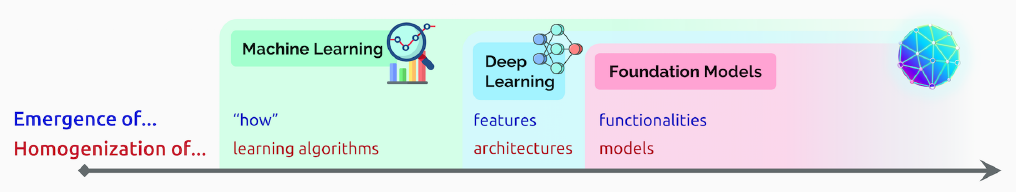
\includegraphics[width=\linewidth]{history} 
 }
\caption{The story of AI \cite{bommasani2021opportunities}.}
\label{Fig:his}
\end{figure}

 Improved classification quality could be achieved by adding metadata (e.g., age, gender, race, skin type, and anatomical location) as inputs for the classifiers. This additional information would be advantageous for dermatologists' decision-making, as Haenssle et al \cite{haenssle2018man} have shown.

The application also allows the tracking of all patient lesions to follow their evolution
over time. Evolution is an important consideration, and it is represented by the E in the ABCD(E) rule. Despite its importance, evolution information will take some years to become available, since a lesion may take some time to increase in size and the patient needs to return to the clinic for ongoing assessment. In this context, when the dermatologist asks the patient whether a lesion has increased  in size or changed in form/appearance, s/he is trying to get information about the lesion’s evolution. It is important to note that clinicians collect this information by questioning patients, which may lead to imprecision and uncertainty. Therefore, clinical data must be used to support the diagnosis. The main information is still coming from the image, however.

Regarding the region of the body where the skin lesion is located, Pacheco et al.\cite{pacheco2020impact} grouped all regions into 15 macro-regions that are more frequently encountered and have more potential to raise skin lesions, as follows: face, scalp, nose, lips, ears, neck, chest, abdomen, back, arm, forearm, hand, thigh, shin, and foot. As skin lesions appear more frequently in certain regions of the body \cite{wolff2009fitzpatrick}, this is an important feature to consider.


% \begin{figure*}
% \centering
% \subfloat[]{\includegraphics[width=2.2in,height=2.9in]{figures/paper1-a.png}%
% \label{Fig:paper1:a}}
% \hspace{0.1em}
% \subfloat[]{\includegraphics[width=2.1in,height=2.9in]{figures/paper1-b.png}%
% \label{Fig:paper1:b}}
% \caption[Pixel resolution plot for six bird paths]{(a) Pixel resolution plot for six bird paths, covered by one camera dome of 3000 pixels capacity, (b) Pixel resolution plot of Path 3, covered by 3 domes of the same capacity. }
% \label{Fig:paper1}
% \end{figure*}

Stanford researchers have called transformers “foundation models” \cite{bommasani2021opportunities}, saying that transformers mark the next stage of AI’s development, what some call the era of transformer AI. As shown in Figure \ref{Fig:his}, the story of AI has been one of the emergence of an increasing number of capabilities and of increasing homogenization. With the introduction of machine learning, how a task is performed emerged (i.e., is inferred automatically) from examples; with deep learning, the high-level features used for prediction emerged; and with foundation models, even advanced functionalities such as in-context learning emerged. At the same time, machine learning homogenizes learning
algorithms (e.g., logistic regression), deep learning homogenizes model architectures (e.g., convolutional neural networks), and foundation models homogenize the model itself (e.g., GPT-3 \cite{brown2020language}).

With its generative pre-trained transformer (GPT), the OpenAI lab \cite{brown2020language} showed that a larger transformer is better than a smaller one. The latest version, GPT-3, has 175 billion parameters, up from 1.5 billion for GPT-2. With this extra heft, GPT-3 can respond to a user’s query even on tasks it was not specifically trained to handle. It is already being used by companies  such as Cisco, IBM, and Salesforce. Figure \ref{Fig:GTC} shows the training computed with different AI models from 2012 to 2022.

\begin{figure}
\centerline{
 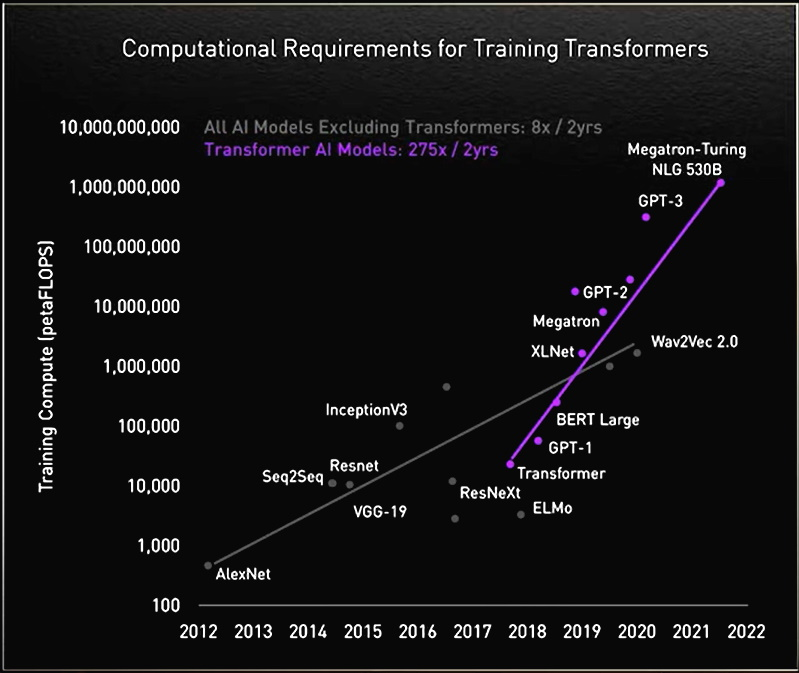
\includegraphics[width=\linewidth]{Transformer-size-timeline-GTC} 
 }
\caption{In the race for higher performance, transformer models have grown larger \cite{whattran}.}
\label{Fig:GTC}
\end{figure}

\section{Summary and findings}

I am eager to develop a decision-support system for dermatologists and other healthcare professionals who found the dermatoscopic technique challenging. It found that addressing class imbalance using loss balancing improved network performance. The work aimed to develop models for classifying skin lesions in dermoscopic images by using a deep learning model. By the end of this work, a hybrid model had been developed. This model uses the Resnet-50 + Transformer networks as the architecture for the deep learning model. A dataset of dermoscopic
images, provided by ISIC2018, has been utilized to train and evaluate the performance of the hybrid model on dermoscopic data. 

Nevertheless, there are some limitations that should be acknowledged.
\begin{itemize} \label{sec.lim}
    \item First, the trained models have not been deployed in clinical practice, but are still in the stage of scientific experimentation.
    \item Due to resource constraints, the model was not trained with the latest backbone or compared with the state-of-the-art models.
    \item All experiments were conducted separately and using different datasets, so the task of conducting all methods using the same dataset is not complete.
    \item This study was limited to the classification of seven skin disorders. It will be necessary to expand the repertoire of skin images to include other cutaneous tumors and normal skin types,  thereby reducing the false-positive rate when using deep learning algorithms in real clinical practice.
    \item Because of its rare incidence in Asians, the number of melanomas in the dataset was insufficient for our analysis, and many of the melanomas that are included were diagnosed at a late stage.
    \item Although the ISIC challenge database is large, it contains many repeated data, so a high-quality database for research on disease classification remains to be created.
\end{itemize}